\documentclass{article}
\usepackage[T1]{fontenc}
\usepackage{lmodern}
\usepackage{graphicx}
\usepackage{amsmath,amssymb}
\usepackage[a4paper,margin=2cm]{geometry}
\usepackage[absolute,overlay]{textpos}
\setlength{\TPHorizModule}{1mm}
\setlength{\TPVertModule}{1mm}
\usepackage[indonesian]{babel}
\usepackage{hyperref}
\setlength{\emergencystretch}{2em}
% unit: Halaman 2

\begin{document}

% === Halaman 2 (python/native) ===

Algoritma Kriptografi Knapsack

• Merupakan salah satu algoritma kriptografi kunci-publik awal yang ditemukan oleh Ralph 

Merkle dan Martin Hellman pada 1978.

• Disebut juga algoritma Merkle-Hellman

2

Merkle, Hellman, dan Diffie

% deskripsi: gambar native xref 29
\noindent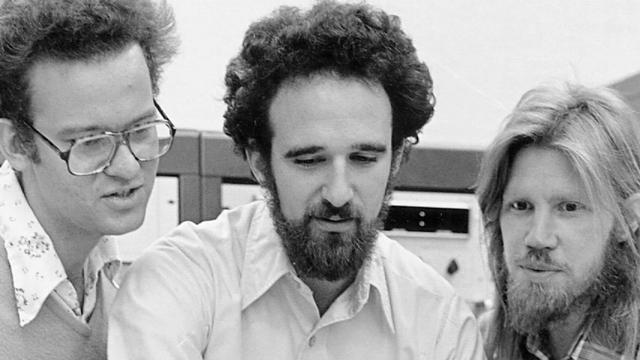
\includegraphics[width=0.85\textwidth]{../../images/python/page_002_img_01.jpeg}

\end{document}
